\chapter{Charge Readout Planes}
\label{ch:fddp-CRP}

%%%%%%%%%%%%%%%%%%%%%%%%%%%%%%%%%%%%%%%%%%%%%%%%%%%%%%%%%%%%%%%%%%%%
\section{Charge Readout Planes (CRP) Overview}
\label{sec:fddp-crp-ov}


%%%%%%%%%%%%%%%%%%%%%%%%%%%%%%%%%
\subsection{Introduction}
\label{sec:fddp-crp-intro}

In the dual-phase LArTPC concept, the ionization electrons are multiplied in avalanches 
occurring inside detectors, the Large Electron Multipliers (LEMs), located in the argon gas 
phase above the liquid argon level. The drift field of the TPC brings the electrons up to the liquid argon surface where they can  be   
extracted into the gas using a 2-kV/cm electric field defined across the liquid-gas interface.
This extraction field is applied between a submersed extraction
grid (stainless steel wires tensioned in both $x$ and $y$
directions) and the bottom side of the LEMs.
The LEMs are printed circuit boards oriented horizontally, with
conductive layers (electrodes) on the top and bottom surfaces, and many holes drilled
through. The holes form a micro-pattern structure within which the amplification occurs.  
By applying voltages across the two
electrodes of the LEM, a 30-kV/cm electric field region is defined in the holes\cite{Bondar:2008yw}.
Electrons transiting these high electric field regions in the holes trigger Townsend multiplication in the
pure argon gas.


The amplified charge is then collected and recorded on a 2D anode
consisting of two sets of 3.125-mm-pitch gold-plated copper strips that provide the $x$
and $y$ coordinates (and thus two views) of the event.

Typical electric fields between each stage of the readout are
illustrated in Figure~\ref{fig:setup}. Table~\ref{tab:crp_dist} shows
the inter-stage distance and the tolerances required to obtain
uniformity of gain to within $\sim$5\%.
\begin{dunefigure}[Dual-phase readout]{setup}{Illustration of the electric fields in the amplification region of a dual-phase LArTPC. The simulated field lines in dark blue indicate the paths followed by the drifting charges (without diffusion).}
 %\includegraphics[width=.8\textwidth]{double_phase_principle.pdf}  
\end{dunefigure}
\begin{dunetable}[Interstage distances and electric field settings of the dual-phase readout components]{lp{2cm}p{2cm}l}{crp_dist}{Interstage distances and electric field settings of the dual-phase readout components.} 
 Component & Distance [mm] & Tolerance [mm] & Electric field [kV/cm]  \\ \toprowrule
 Anode-LEM top electrode  & 2 & 0.1 & 5\\ \colhline
 LEM top-bottom electrode   & 1 & 0.01 & 30-35\\ \colhline
 LEM bottom electrode-grid        & 10 & 1 & 2 (in LAr) and 3 (in GAr)\\
 \end{dunetable}

The extraction grid, LEM and anode are assembled into three-layered ``sandwiches'' with precisely defined inter-stage distances and inter-alignment,  which are then connected together horizontally into
modular units of area \num{9}~m$^2$. These units are called Charge Readout Planes (CRPs).

The Charge Readout Planes provide ...
The system includes (whatever it includes), as shown in Figure~\ref{fig:figure-label-crp1}.... 



\begin{dunefigure}[optional caption for LoF]{fig:figure-label-crp1}
{required full caption (Credit: xyz)}
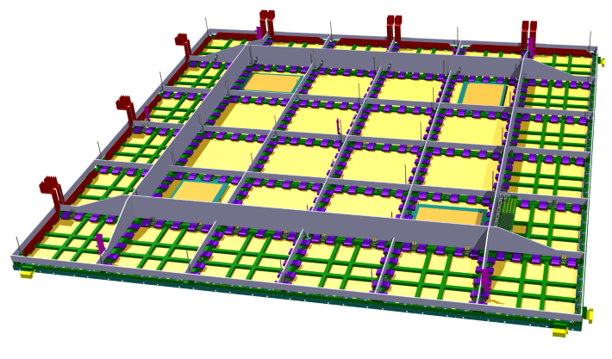
\includegraphics[width=0.8\textwidth]{CRP-fig1.png}
\end{dunefigure}

The operating principle is illustrated in Figure~\ref{fig:figure-label-crp2}... (add figure)


%%%%%%%%%%%%%%%%%%%%%%%%%%%%%%%%%%%%%
\subsection{Design Considerations}
\label{sec:fddp-crp-des-consid}

Each CRP is an independent detector element that performs charge
extraction, multiplication and collection, and has its own high
voltage system and independent signal feedthroughs. The entire area of
the LEM and anode in a CRP is active.

The LEM and corresponding anode are mounted in units of 50$\times$50~cm$^2$, called
LEM/Anode Sandwich (LAS) modules, before being assembled with an extraction
grid into a CRP. Each
anode in a LAS is segmented in 50-cm long $x$ and $y$ strips . Adjacent LAS anodes
are bridged together to form readout strips of the required length by
connecting short flat cables to KEL connectors soldered onto the top
sides of the anodes. The signals from the last anode in each 
strip chain are brought to feedthroughs
mounted on the other side of the front-end electronics embedded inside
dedicated signal-feedthrough chimneys using 50-cm-long flat cables.


Each CRP is independently hung from the vessel deck through its three
suspension feedthroughs. It has its own high voltage system and 
independent signal and slow-control feedthroughs.
The Charge Readout Planes design must enable... 
...

\fixme{Anne suggests: Within this section add ref to requirements document  when it's ready, and maybe list the most important half dozen in a table here). E.g.,}  

See Table~\ref{tab:crpphysicsparams} for a list of physics parameters that drive the design...

\begin{dunetable}
[Important parameters for the CRP system design]
{p{0.8\textwidth}}
{tab:crpphysicsparams}
{Important parameters for the CRP system design}   
Parameter \\ \toprowrule
  \\ \colhline
   \\ \colhline
 ...\\ 
\end{dunetable}

\fixme{By the end of the volume, for every requirement listed in this section, there should exist an explanation of how it will be satisfied.}


%%%%%%%%%%%%%%%%%%%%%%%%%%%%%%%%
\subsection{Scope}
\label{sec:fddp-crp-scope}

The scope of the Charge Readout Planes includes the continued procurement of materials for, and the fabrication, testing, delivery and installation of the following systems: 

\fixme{Whatever the items are...}

\begin{itemize}
\item  
\item  ...
\end{itemize}



%%%%%%%%%%%%%%%%%%%%%%%%%%%%%%%%%%%%%%%%%%%%%%%%%%%%%%%%%%%%%%%%%%%%
\section{CRP Design}
\label{sec:fddp-crp-design}


\fixme{Include an image of the subsystem, indicating its parts. Show how the system fits into the overall system).}

%%%%%%%%%%%%%%%%%%%%%%%%%%%%%%%%%%%
\subsection{Mechanical structure}
\label{sec:fddp-crp-mechanics}

%%%%%%%%%%%%%%%%%%%%%%%%%%%%%%%%%%%
\subsection{Extraction grid}
\label{sec:fddp-crp-grid}
The extraction grid consists of 100 μm diameter stainless steel wires tensioned in both x and y directions over the entire 3-m length/width of the CRP with 3.125 mm pitch. They are soldered into groups of 64 on independent wire-tensioning pads oriented perpendicularly to the side of the CRP frame. Each wire-tensioning pad consists of a printed circuit board (PCB) for HV-connection that is fixed very precisely to a mechanical wire holder. The PCB has 32 soldering pads with 200- μm grooves for precise positioning of the wires. During the wire-soldering process each wire is tensioned and positioned in a groove. The PCB is then mounted on the wire holder and the tension of the group of 32 wires
can be precisely adjusted by pushing the holder against the CRP’s FR4 frame with two screws. The wires, 3 m long in both x and y directions, have their sags minimized to 0.1 mm thanks to x and y oriented supporting comb-teeth blades  inserted between anode planes of 1 m×1 m size. The array of blades penetrates the liquid surface and has the additional benefit of maintaining the liquid level still.

%%%%%%%%%%%%%%%%%%%%%%%%%%%%%%%%%%%
\subsection{Large Electron Multiplier (LEM)}
\label{sec:fddp-crp-lem}
Each LEM is built from a 1-mm-thick copper-clad epoxy PCB with 500 μm diameter holes drilled through, surrounded by a 40-μm dielectric rim. The holes are arranged in a honeycomb pattern with a pitch of 800 μm, resulting in about 200 holes per cm2
and O(500,000) holes over the entire 50×50 cm2 area. The holes provide confinement for the UV photons produced during the avalanche process and thus act as a mechanical quencher to prevent photon feedback. This property makes the LEM suitable for operation in ultra-pure argon vapor without the addition of a quenching gas.

%%%%%%%%%%%%%%%%%%%%%%%%%%%%%%%%%%%
\subsection{Anode}
\label{sec:fddp-crp-anode}
Each 50×50 cm2 anode is manufactured from a single multilayer Printed Circuit Board (PCB). The readout strips for both x and y views consist of a pattern of gold-plated
copper tracks with a 3.125-mm readout pitch. The two views have superimposed track patterns
that are electrically insulated from one another. Electrical insulation in the points where the x and y tracks would superimpose is achieved by having tracks crossing over and under each other using a system of vias between the top and bottom layers of the PCB.
The design of the track patterns forming the strips is such that both x and y views collect the same amount of charge, independent of the angle of charged-particle tracks with respect to the readout strip orientation. The tracks pattern should then ensure a uniform and isotropic coverage of the strip surface while minimizing the strip capacitance. These criteria have driven a thorough design optimization. 

%%%%%%%%%%%%%%%%%%%%%%%%%%%%%%%%%%%
\subsection{Instrumentation}
\label{sec:fddp-crp-instr}

%%%%%%%%%%%%%%%%%%%%%%%%%%%%%%%%%%%
\subsection{Suspension system and drive}
\label{sec:fddp-crp-suspension}
Three suspension feedthroughs are arranged as an equilateral triangle whose barycenter coincides with that of the CRP; they suspend the CRP at the required position and precisely adjust the CRP level with respect to the liquid argon surface

%%%%%%%%%%%%%%%%%%%%%%%%%%%%%%%%%%%
\subsection{Quality Assurance}
\label{sec:fddp-crp-qa}

%%%%%%%%%%%%%%%%%%%%%%%%%%%%%%%%%%%%%%%%%%%%%%%%%%%%%%%%%%%%%%%%%%%%
\section{Production and Assembly}
\label{sec:fddp-crp-prod-assy}

%%%%%%%%%%%%%%%%%%%%%%%%%%%%%%%%%%
\subsection{G10 and Invar frame production}
\label{sec:fddp-crp-frame}

%%%%%%%%%%%%%%%%%%%%%%%%%%%%%%%%%%
\subsection{LEM and anode production}
\label{sec:fddp-crp-LASprod}

%%%%%%%%%%%%%%%%%%%%%%%%%%%%%%%%%%
\subsection{Tooling}
\label{sec:fddp-crp-tooling}


%%%%%%%%%%%%%%%%%%%%%%%%%%%%%%%%%
\subsection{Assembly Procedures}
\label{sec:fddp-crp-assy}


%%%%%%%%%%%%%%%%%%%%%%%%%%%%%%%%%%%%%%%%%%%%%%%%%%%%%%%%%%%%%%%%%%%%
\section{Interfaces}
\label{sec:fddp-crp-intfc}

\fixme{Include an image of each interface in appropriate section.}

%%%%%%%%%%%%%%%%%%%%%%%%%%%%%%%%%%%
\subsection{TPC Electronics}
\label{sec:fddp-crp-intfc-elec}


%%%%%%%%%%%%%%%%%%%%%%%%%%%%%%%%%%%
\subsection{Instrumentation and HV Feed-through flanges}
\label{sec:fddp-crp-intfc-FT}

%%%%%%%%%%%%%%%%%%%%%%%%%%%%%%%%%%%
\subsection{Cryostat/Detector Support Structure}
\label{sec:fddp-crp-intfc-support}

%%%%%%%%%%%%%%%%%%%%%%%%%%%%%%%%%%%
\subsection{HV/Slow control}
\label{sec:fddp-crp-intfc-HV-slowcontrol}


%%%%%%%%%%%%%%%%%%%%%%%%%%%%%%%%%%%%%%%%%%%%%%%%%%%%%%%%%%%%%%%%%%%%
\section{Installation, Integration and Commissioning}
\label{sec:fddp-crp-install}

%%%%%%%%%%%%%%%%%%%%%%%%%%%%%%%%%%%%
\subsection{Transport and Handling}
\label{sec:fddp-crp-install-transport}


%%%%%%%%%%%%%%%%%%%%%%%%%%%%%%%%%%%
\subsection{Integration with (electronics, ???)}
\label{sec:fddp-crp-install-pd-???}


%%%%%%%%%%%%%%%%%%%%%%%%%%%%%%%%%%%
\subsection{Calibration?}
\label{sec:fddp-crp-install-calib}



%%%%%%%%%%%%%%%%%%%%%%%%%%%%%%%%%%%%%%%%%%%%%%%%%%%%%%%%%%%%%%%%%%%%
\section{Quality Control}
\label{sec:fddp-crp-qc}

%%%%%%%%%%%%%%%%%%%%%%%%%%%%%%%%%%%%
\subsection{Protection and Assembly (Local)}
\label{sec:fddp-crp-qc-local}


%%%%%%%%%%%%%%%%%%%%%%%%%%%%%%%%%%%
\subsection{Post-factory Installation (Remote)}
\label{sec:fddp-crp-qc-remote}



%%%%%%%%%%%%%%%%%%%%%%%%%%%%%%%%%%%%%%%%%%%%%%%%%%%%%%%%%%%%%%%%%%%%
\section{Safety}
\label{sec:fddp-crp-safety}

%%%%%%%%%%%%%%%%%%%%%%%%%%%%%%%%%%%
% add subsections and labels if needed \subsection{}
%\label{sec:fddp-crp-safety-}


%%%%%%%%%%%%%%%%%%%%%%%%%%%%%%%%%%
%\subsection{}
%\label{sec:fddp-crp-safety}



%%%%%%%%%%%%%%%%%%%%%%%%%%%%%%%%%%%%%%%%%%%%%%%%%%%%%%%%%%%%%%%%%%%%
\section{Organization and Management}
\label{sec:fddp-crp-org}

%%%%%%%%%%%%%%%%%%%%%%%%%%%%%%%%%%%
\subsection{CRP Consortium Organization}
\label{sec:fddp-crp-org-consortium}


%%%%%%%%%%%%%%%%%%%%%%%%%%%%%%%%%%
\subsection{Planning Assumptions}
\label{sec:fddp-crp-org-assmp}


%%%%%%%%%%%%%%%%%%%%%%%%%%%%%%%%%%%
\subsection{WBS and Responsibilities}
\label{sec:fddp-crp-org-wbs}

%%%%%%%%%%%%%%%%%%%%%%%%%%%%%%%%%%
\subsection{High-level Cost and Schedule}
\label{sec:fddp-crp-org-cs}














